% Created 2022-11-17 Thu 17:17
% Intended LaTeX compiler: pdflatex
\documentclass[a4paper,11pt]{article}
\usepackage[utf8]{inputenc}
\usepackage[T1]{fontenc}
\usepackage{graphicx}
\usepackage{longtable}
\usepackage{wrapfig}
\usepackage{rotating}
\usepackage[normalem]{ulem}
\usepackage{amsmath}
\usepackage{amssymb}
\usepackage{capt-of}
\usepackage{hyperref}
\usepackage[margin=1in]{geometry}
\usepackage{titlesec}
\usepackage{caption}
\usepackage{subcaption}
\usepackage{lipsum}
\author{Varghese Reji}
\date{}
\title{Classical and Quantum Optics\\\medskip
\large Assignment-2 Answers}
\hypersetup{
 pdfauthor={Varghese Reji},
 pdftitle={Classical and Quantum Optics},
 pdfkeywords={},
 pdfsubject={},
 pdfcreator={Emacs 28.2 (Org mode 9.5.5)}, 
 pdflang={English}}
\begin{document}

\maketitle

\section*{Problem 1}
\label{sec:org0303043}
In the Einstein analysis we assume that the light radiation has a broad spectrum compared to the transition line. Let us now consider the contrary situation in which the spectral width of the light beam is much smaller than the linewidth of the transition. This is the kind of situation that occurs when a narrow-band laser beam interacts with as atom, inside a laser cavity or externally.
\begin{description}
\item[{(a)}] Explain why it is appropriate to write the spectral energy intensity of the beam as:
$$u(\omega') = u_\omega\delta(\omega'-\omega)$$
where \(\omega\) is the angular frequency of the beam, \(u_\omega\) is its energy density in \(Jm^{-3}\), and \(\delta(x)\) is the Dirac Delta function.
\item[{(b)}] Let us assume that the frequency dependence of the absorption probability follows the spectral lineshape function g\textsubscript{\(\omega\)}(\(\omega\)). This implies that the Einstein \(B\) coefficients will also vary with frequency. Explain why it is appropriate to write the frequency dependence of the Einstein \(B_{12}\) coefficient as:
$$B_{12} = \frac{g_2}{g_1} \frac{\pi^2c^3}{\hbar n^3\omega'^3} \frac{1}{\tau} g_{\omega}(\omega')$$
\item[{(c)}] Hence show that the total absorption rate defined as
$$W_{12} = N_1\int_{0}^{\infty} B_{12}(\omega') u(\omega')d\omega'$$
is given by:
$$W_{12} = N_1 \frac{g_2}{g_1} \frac{\pi^2c^3}{\hbar n^3\omega'^3} \frac{1}{\tau} u_{\omega}g_{\omega}(\omega')$$
\item[{(d)}] Repeat the arguement to show that the total stimulated-emission rate is given by:
$$W_{21} = N_2 \frac{\pi^2c^3}{\hbar n^3\omega'^3} \frac{1}{\tau} u_{\omega}g_{\omega}(\omega')$$
\end{description}

\section*{Problem 2}
\label{sec:orgfc0a9ca}

\newpage
\section*{Problem 3}
\label{sec:org759b8e9}
Calculate the fraction of energy of a 00-mode laser beam with beam radius \(w\) within a distance \(w\) from the beam centre.
\subsection*{Solution}
\label{sec:org5bbf05d}
The electric field at a distance for 00-mode is given by

$$\mathcal{E}=\mathcal{E}_0\exp\left(-\frac{r^2}{w^2}\right)$$

Energy density of an electric field is given by, \(u=\frac{1}{2}\epsilon_0\mathcal{E}^2\). 

Then, total energy in a particular distance \(r\) is given by,

$$E(r) = \int_V udV = \pi \epsilon_0 \mathcal{E_0}^2\int_0^r e^{-\frac{2r'^2}{w^2}} r'dr' $$ 

$$=\pi\epsilon_0\frac{w^2\left(1-\exp\left( \frac{-2 r^2}{w^2}\right)\right)}{4}$$

So, the fraction of energy in distance \(w\)

$$\frac{E(w)}{E(\infty)} = 1-e^{-2}=0.864 = 86.4\%$$

\section*{Problem 5}
\label{sec:org07d70a8}
Estimate the Doppler and collision line widths of emission from \(H_2O\) molecules at \(\lambda = 0.5\mu m\), at 300K and atmospheric pressure. Assume the collision cross-section to be the same as the geometrical size of the molecule.

\subsection*{Solution}
\label{sec:org7551358}
Given, \(\lambda = 0.5\mu m\), T=300K.

Let us consider the maximum possible geometrical area, which is in the plane perpendicular to \(z\) axis which pass through the oxygen atom. The angle between hydrogen atoms is \(104.45^o\), and length of one handle is \(l=95.84 pm\). \footnote{\url{https://en.wikipedia.org/wiki/Chemical\_bonding\_of\_water}}.And Atmospheric pressure is P=101325 Pa.

From Kinetic theory of gasses, we will get

\begin{equation}
\label{eq:org609bada}
\tau_{col} \sim \frac{1}{\sigma P} \left(\frac{\pi m k_B T}{8}\right)^{\frac{1}{2}}
\end{equation}

m = 2m\textsubscript{H} + m\textsubscript{O} = 17m\textsubscript{H};
\(\sigma\) = \(\pi\) l\textsuperscript{2} \(\sin\)(104.45) = 2.70596603659\texttimes{} 10\textsuperscript{-20} m\textsuperscript{2} 

\(\therefore\)
$$\tau_{col} = 2.47784340277\times10^{-9}s$$

Then, linewdith, $$\Delta\omega_{col} = 2.53574753762\times10^9 s= 2.526 GHz$$

The linewidth by doppler broadening is given by the formula,

\begin{equation}
\label{eq:orgb4f6f79}
\Delta\omega_{Doppler} = \frac{4\pi}{\lambda} \left(\frac{2 k_B T  \ln 2}{m}\right)^{\frac{1}{2}} 
\end{equation}

Then, we will get,

$$\Delta\omega_{Doppler} = 1.13001722187\times 10^{10} = 11.30 GHz$$

\newpage
\section*{Problem 6}
\label{sec:orgfdf335e}
Monochromatic light is scattered at \(90^o\) from a cell containing \(10^{-16}\) g particles in suspension at 300K. Estimate the coherence time and linewidth of the scattered light.
\subsection*{Solution}
\label{sec:org4439522}

The wavelength is not specified. So, assume that \(\lambda = 500nm\). T=300K
We can consider the scattering in this case like reflection from a moving mirror. The particles in this is in thermal motion. So, using kinetic theory, the kinetic energy of each particle in each direction is \(\frac{1}{2}k_BT\).

Here, the scattering is in \(90^o\). So, we can consider the line of sight along the path of reflected ray. We need to consider the motion of particle in that direction only. Let us take that direction as \(x\). Then, we can write,

$$\frac{1}{2} m v_x^2 = \frac{1}{2} k_B T$$.

Then, $$v_x = \sqrt{\frac{k_BT}{m}} = 2.034\times 10^{-1} m/s = 20.34cm/s$$

The Doppler shift can be written as

$$\frac{\delta\lambda}{\lambda} = \frac{v_x}{c} = 6.782\times10^{-10}$$

Then, 

$$\delta\lambda = \frac{v_x\lambda}{c} = 3.3911\times 10^{-16} m = 3.391\times 10^{-7}nm $$

The coherence time is given by the formula

$$\tau_c = \frac{\lambda^2}{c\delta \lambda} = \frac{\lambda}{v_x}$$

Then,

$$\tau_c = 1.667\times 10^{-15} = 1.667 fs $$

\newpage
\section*{Problem 7}
\label{sec:orgc8bb4f5}
Several output modes of a laser, indicated by the small integer m which lies between, say, +5 and –5, are represented by the waves 
\begin{equation}
E_n=a\exp\left[-i[(\omega_0+n\omega_1)t+\phi_n]\right]
\end{equation}
where \(\omega_1\) is the mode-spacing frequency. To illustrate mode-locking, calculate the wave resulting from superposition of these modes when (a) \(\phi_n\) is a random variable and (b) all \(\phi_n = 0\). (It is convenient to do this by computer.) 
\subsection*{Solution}
\label{sec:org7741e73}
The solution of this is done in python. You can see the code \href{https://github.com/varghesereji/Coursework\_assignments/blob/main/CQO/Ass\_2/Problem\_7\_answer\_code.py}{here.}
\begin{description}
\item[{(a)}] In this case, values of \(\phi\) is random.  The mode-locked pulses will be as shown in the figure below.
\end{description}
\begin{center}
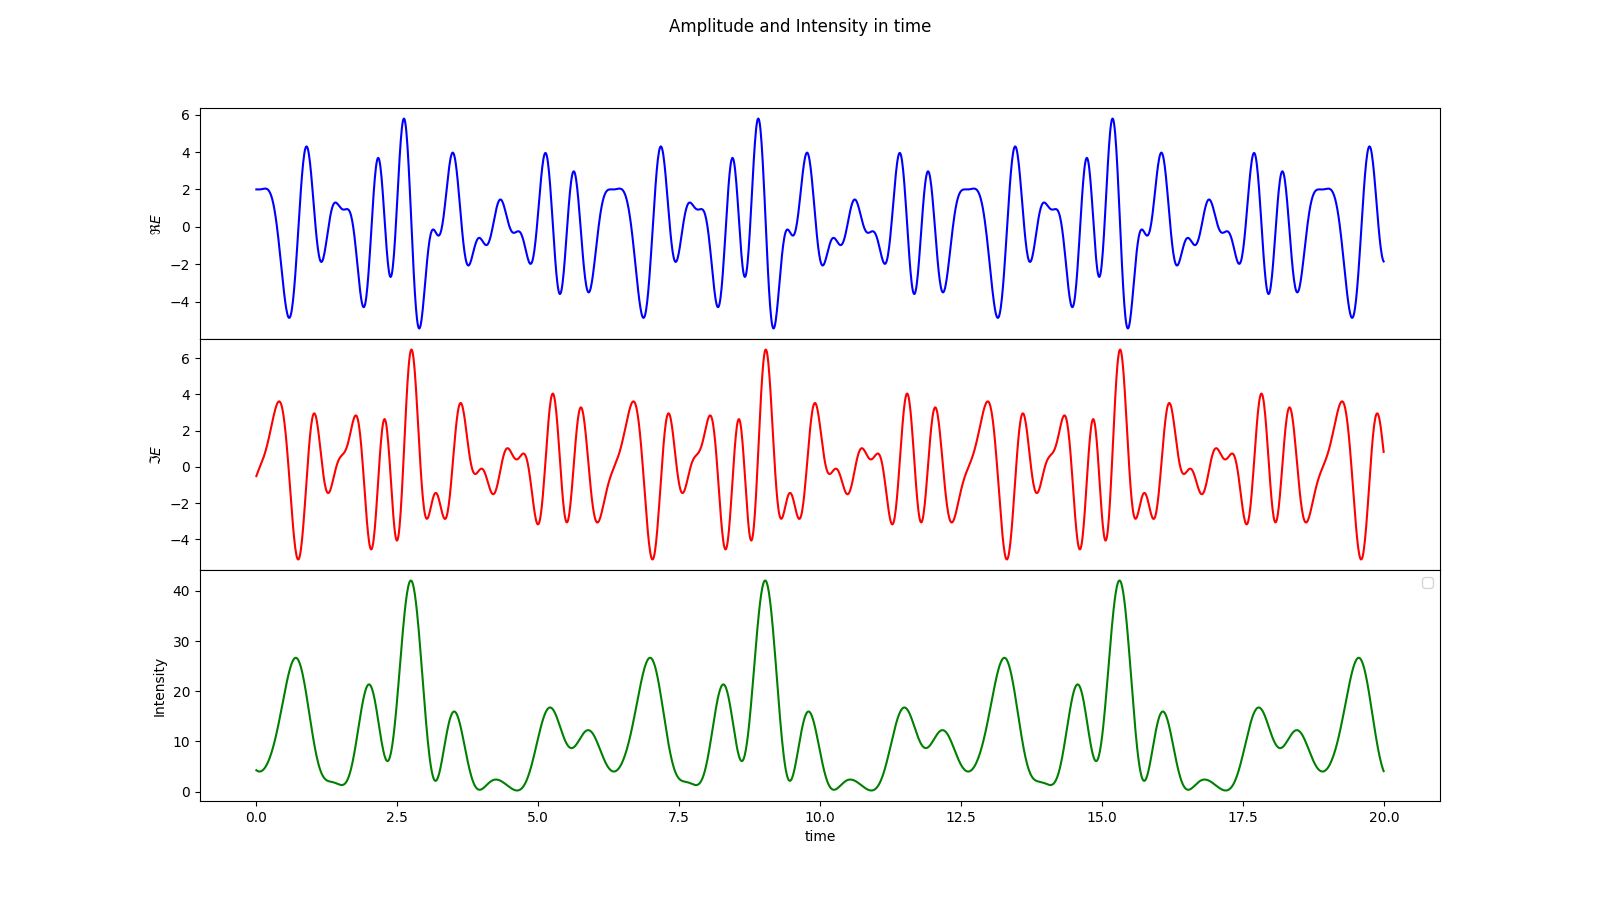
\includegraphics[width=.9\linewidth]{pr_7_a.png}
\end{center}
\begin{description}
\item[{(b)}] Here, \(\phi\) is 0. The pulses is shown in the figure below.
\end{description}
\begin{center}
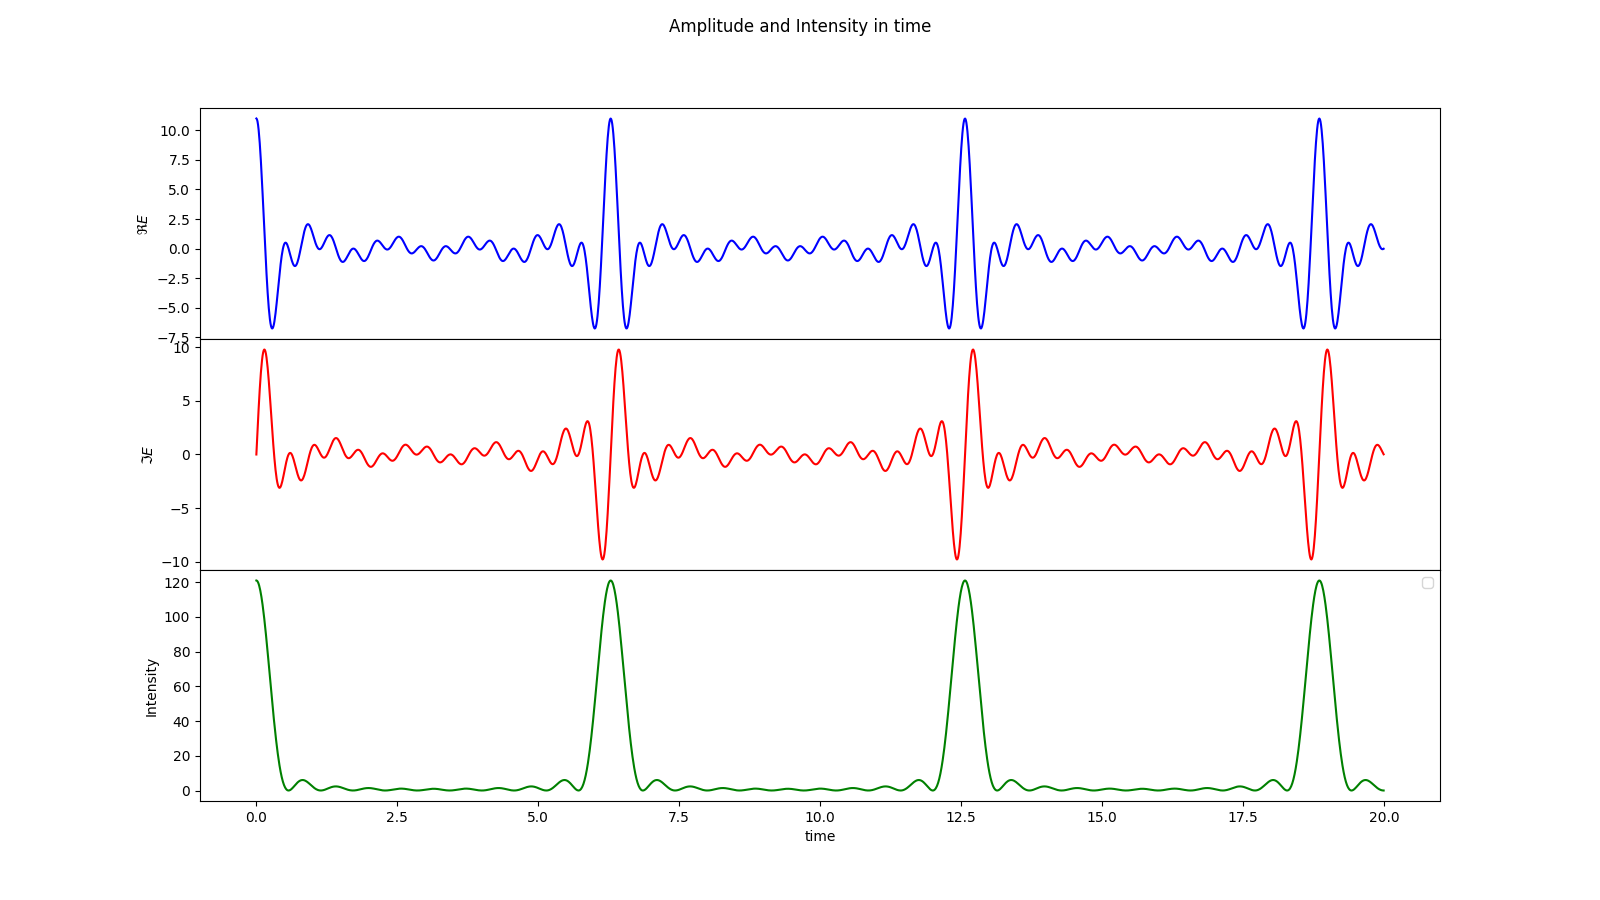
\includegraphics[width=.9\linewidth]{pr_7_b.png}
\end{center}

\newpage

\section*{Problem 8}
\label{sec:org0e387b5}
A material has six energy levels A to F at 2, 1.9, 1.7, 1.6, 1.1 and 0.4 eV above the ground state, G. The time constants for the various possible transitions in nanoseconds are shown in figure (Now adding here.) Suggest possible lasers working with this material, and give the pump and output wavelendths of each one.
\subsection*{Solution}
\label{sec:org515a892}

For a laser, we have to satisfy condition to happen the lasing.
\begin{description}
\item[{(a)}] The lowest level is the ground state
\item[{(b)}] Uppermose state must be connected to the ground state by a short time constant if optical pumping is to be used.
\item[{(c)}] One pair of levels, which will be lasing levels must be connected weakly, i.e. the time constant for transitions between them must be long compared to the others involved
\item[{(d)}] The upper laser level must not have a faster competing transition to another level, excluting the ground state of optical pumping is used.
\end{description}

\subsubsection*{Energy levels}
\label{sec:org30509e7}
\begin{center}
\begin{tabular}{|c|c|c|c|c|c|c|c|}
\hline
Level & A & B & C & D & E & F & G\\
\hline
Energy from G(eV) & 2 & 1.9 & 1.7 & 1.6 & 1.1 & 0.4 & 0\\
\hline
\end{tabular}
\end{center}

\subsubsection*{Time constants between different levels in nanoseconds.}
\label{sec:orga27d2ff}
\begin{center}
\begin{tabular}{|c|c|c|c|c|c|c|}
\hline
B & 0 & - & 50 & 50 & 10\textsuperscript{4} & 0\\
\hline
C & 10 & 50 & - & 10\textsuperscript{4} & 10\textsuperscript{4} & 0\\
\hline
D & 0 & 50 & 10\textsuperscript{4} & - & 0 & 10\textsuperscript{4}\\
\hline
E & 0 & 10\textsuperscript{4} & 10\textsuperscript{4} & 0 & - & 100\\
\hline
F & 0 & 0 & 0 & 10\textsuperscript{4} & 100 & -\\
\hline
G & 10 & 10 & 0 & 0 & 10\textsuperscript{4} & 10\\
\hline
 & A & B & C & D & E & F\\
\hline
\end{tabular}
\end{center}

The lasing will happen when the time constants are sufficiently high. So, we need to look only for such cases from the above table. This condition had been satisfied in 5 cases with time constant \(10^{5} ns\). Those are,  C\(\rightarrow\) D, B\(\rightarrow\) E, C\(\rightarrow\) E, C\(\Rightarrow\) F and E\(\rightarrow\) G.

\subsubsection*{Levels for lasing}
\label{sec:org2525d2b}

\begin{center}
\begin{tabular}{llrrrrl}
\hline
Higher & Lower & Em\textsubscript{2} & Em\textsubscript{1} & Em\textsubscript{2}-Em\textsubscript{1} & \(\lambda\) & Comment\\
 &  & (eV) & (eV) & (eV) & (\(\mu\) m) & \\
\hline
C & D & 1.7 & 1.6 & 0.1 & 12.42375 & 4L\\
C & F & 1.7 & 0.4 & 1.3 & 0.95567308 & 4L\\
C & E & 1.7 & 1.1 & 0.6 & 2.070625 & 4L\\
B & E & 1.9 & 1.1 & 0.8 & 1.5529688 & 3L\\
E & G & 1.1 & 0 & 1.1 & 1.1294318 & 3L\\
\hline
\end{tabular}
\end{center}


To reach this higher metastable state, pumping level should be larger than that. Now, let us look on the required pumping levels and pumping energy. The time constant for this should be low.

\subsubsection*{Pumping wavelengths}
\label{sec:org8a901c5}
\begin{center}
\begin{tabular}{lllrrrrl}
\hline
Upper & Higher & Lower & E\textsubscript{2} & E\textsubscript{1} & E\textsubscript{2}-E\textsubscript{1} & \(\lambda\) & Comment\\
Metastable & Pumping & Pumping & (eV) & (eV) & (eV) & (micron) & \\
State & level & level &  &  &  &  & \\
\hline
C & A & G & 2 & 0 & 2 & 0.6211875 & 4L\\
C & B & G & 1.9 & 0 & 1.9 & 0.65388158 & 4L\\
B & B & G & 1.9 & 0 & 1.9 & 0.65388158 & 3L\\
B & B & C & 1.9 & 1.7 & 0.2 & 6.211875 & 3L\\
B & B & D & 1.9 & 1.6 & 0.3 & 6.211875 & 3L\\
E & E & F & 1.1 & 0.4 & 0.7 & 1.7748214 & 3L\\
\hline
\end{tabular}
\end{center}

\subsubsection*{Possible Lasing Actions}
\label{sec:org991b4e5}
\begin{center}
\begin{tabular}{|c|c|c|c|c|c|c|c|c|}
\hline
E\textsubscript{1} & E\textsubscript{2} & Em\textsubscript{2} & Em\textsubscript{1} & \(\tau\) & \(\tau\) & Output & pump & Comment\\
 &  &  &  & pumping & lasing & \(\lambda\) & \(\lambda\) & \\
 &  &  &  & (ns) & (ns) & (\(\mu\) m) & (\(\mu\) m) & \\
\hline
G & A & C & D & 10 & 10000 & 12.42375 & 0.6211875 & 4L\\
G & B & C & D & 10 & 10000 & 12.42375 & 0.65388158 & 4L\\
G & A & C & F & 10 & 10000 & 0.95567308 & 0.6211875 & 4L\\
G & B & C & F & 10 & 10000 & 0.95567308 & 0.65388158 & 4L\\
G & A & C & E & 10 & 10000 & 2.070625 & 0.6211875 & 4L\\
G & B & C & E & 10 & 10000 & 2.070625 & 0.65388158 & 4L\\
G & B & B & E & 10 & 10000 & 1.5529688 & 0.65388158 & 3L\\
C & B & B & E & 50 & 10000 & 1.5529688 & 6.211875 & 3L\\
D & B & B & E & 50 & 10000 & 1.5529688 & 6.211875 & 3L\\
F & E & E & G & 100 & 10000 & 1.1294318 & 1.7748214 & 3L\\
\hline
\end{tabular}
\end{center}
\end{document}